\RequirePackage[2020-02-02]{latexrelease}
\documentclass[twocolumn]{revtex4}

\usepackage[utf8]{inputenc}
\usepackage{lmodern}
\usepackage[T1]{fontenc}
\usepackage{mathtools}
\usepackage{float}
\usepackage{csvsimple}
\providecommand{\abs}[1]{\lvert#1\rvert}
\usepackage{braket}
\providecommand{\eq}[2]{
    \begin{equation}
        #2
    \label{eq:#1}
    \end{equation}
}
\providecommand{\eqgat}[2]{
    \begin{gather}
        #2
    \label{eq:#1}
    \end{gather}
}
\usepackage{amsmath}
\usepackage{amsfonts}
\DeclareMathOperator{\calH}{\mathcal{H}}
\DeclareMathOperator{\calL}{\mathcal{L}}
\DeclareMathOperator{\calN}{\mathcal{N}}
\DeclareMathOperator{\tr}{tr}
\usepackage{fancyhdr}
\usepackage{wrapfig}
\usepackage{graphicx}
% \usepackage[hidelinks]{hyperref}



\begin{document}


\pagestyle{fancy}
\lhead{\bf Entanglement Entropy and Holography}
\rhead{Ferran Rodríguez Mascaró}
\lfoot{Treball de Fi de Grau}
\rfoot{Barcelona, January 2023}


\title{Entanglement Entropy and Holography}
\author{Author: Ferran Rodríguez Mascaró}
\email{ferran.r.m11@gmail.com} %optional
\affiliation{Facultat de F\'{\i}sica, Universitat de Barcelona, Diagonal 645, 08028 Barcelona, Spain.}
\author{Advisor: Pablo Bueno Gómez}
%\date{\today}


\begin{abstract}
    {\bf Abstract:} The AdS/CFT correspondence, also called \textit{holography}, is a physical duality between quantum gravity theories in anti-de Sitter (AdS) spacetimes and certain quantum field theories (QFTs) with conformal symmetry defined in the boundary of such space. The so-called holographic dictionary describes how quantities from each of these theories can be translated into quantities of the other. An important magnitude of the holographic dictionary is the entanglement entropy (EE) of boundary regions. This measures the degree of quantum entanglement between such regions and their complements. In this work, we study various aspects of EE in the holographic context. After a quick review of AdS/CFT and of general aspects of EE in QFT, we introduce the Ryu-Takayanagi formula, which computes the holographic EE of boundary regions in the semiclassical limit of the gravity side of the duality. We perform explicit calculations and general checks of the formula, review its generalizations to account for stringy and quantum corrections, and comment on its relation with black hole thermodynamics and the emergence of gravitational dynamics.
\end{abstract}


\maketitle


\section{Introduction} \label{s:Intro}






\newpage


\section{Holography and AdS/CFT}


\subsection{The Holographic Principle} \label{ss:Holography}

Given a finite space region, one can imagine a process in which matter is continuously added into it. This will make the entropy increase. However, there is a limit to the amount of matter that can be introduced in the region, corresponding to the moment in which a black hole is formed. The entropy of a black hole only depends on its surface area and it is given, in Planck units, by \cite{bekenstein_black_1973, hawking_particle_1975}
\eq{BH}{
    S_\text{BH} = \frac{ A_\text{H} }{ 4 G } \ ,
}
where $A_\text{H}$ is the area of the event horizon of the black hole and $G$ is Newton's gravitational constant. As a consequence, the maximum entropy that a region can contain is given by its area divided by $4G$.

This bound implies that the degrees of freedom inside some region grow with the area of the boundary and not with the volume of the region, as one might have expected. This behaviour leads to the \textit{holographic principle}, which states that in a quantum gravity theory all physics phenomena within some volume must be describable in terms of a theory defined on the boundary of the region \cite{t_hooft_dimensional_2009}.


\subsection{AdS/CFT Correspondence} \label{ss:AdS/CFT}

The \textit{AdS/CFT correspondence}, sometimes simply called \textit{holography} or \textit{gauge/gravity correspondence} \cite{maldacena_large_1999}, is an explicit realization of the holographic principle. It establishes the complete physical equivalence between quantum gravity theories living in anti-de Sitter spacetimes and certain types of conformal quantum field theories (CFTs) living in the boundary of such spacetimes. If the gravitational theory is defined in $(d+1)$ spacetime dimensions, the dual CFT will be defined in $d$ spacetime dimensions and, in a precise sense, the gravity theory will be a ``hologram'' of the CFT. AdS/CFT correspondence allows us to study aspects of each of these theories through the other. The so-called \textit{holographic dictionary} relates quantities (observables) between the gravity theories and their dual CFTs \cite{witten_anti_1998, gubser_gauge_1998}. For example, an empty AdS spacetime with no matter is dual to the vacuum state of the CFT, and an AdS spacetime with a black hole inside corresponds to a thermal state in the CFT.

An anti-de Sitter spacetime is a maximally symmetric spacetime with negative curvature, which solves Einstein's field equations with a negative cosmological constant. The metric of an AdS spacetime of $(d+1)$ dimensions in Poincaré coordinates is \cite{kaplan_lectures_nodate}
\eq{AdS_PP-metric}{
    \mathrm{d} s_{\text{AdS}_{(d+1)}}^2 = \frac{L^2}{z^2} \left( -\mathrm{d} t^2 + \mathrm{d} z^2 + \sum_{i=1}^{d-1} \mathrm{d} x_i^2 \right) \ ,
}
with the time and spatial dimensions $t , x_i \in (-\infty,+\infty)$, an extra dimension $z \in (0,+\infty)$, sometimes called \textit{holographic coordinate}, and where $L$ is the \textit{AdS radius}. Fixing the coordinate $z$, the metric reduces to the one of $d$-dimensional Minkowski spacetime ``weighted'' by the constant factor $1/z^2$. Hence, AdS can be foliate by Minkowski spacetimes living at different values of $z$.

\begin{wrapfigure}[13]{r}{0.26\textwidth}
    \centering
    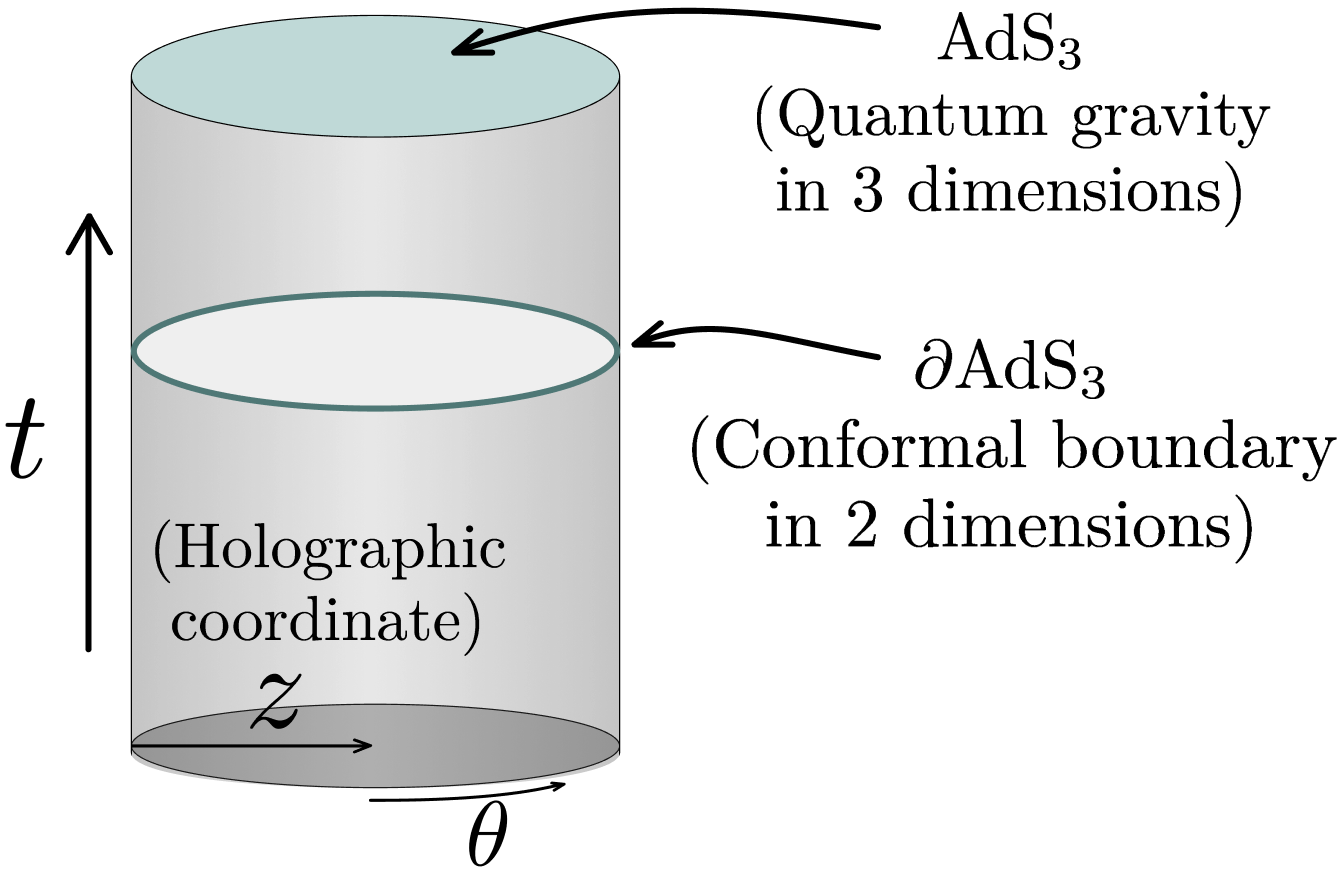
\includegraphics[width=0.26\textwidth]{../imatges/AdS_Cylindric.png}
\caption{AdS$_3$ spacetime. In the conformal boundary lives the CFT$_2$.}
\label{fig:AdS}
\end{wrapfigure}

AdS$_{d+1}$ spacetimes can be represented as cylinders where every slice corresponds to a constant time and where the extra dimension $z$ grows radially towards the center of the cylinder \cite{hawking_large_2008}. Each slice has a $d$-dimensional boundary $\partial$AdS$_{(d+1)}$ where the CFT$_d$ lives (Fig.~\ref{fig:AdS}).

Conformal field theories, on the other hand, are QFTs that are invariant under conformal transformations. These are angle-preserving transformations which leave the metric invariant up to an overall factor \cite{ginsparg_applied_1988}. In particular, the Poincaré group is a subgroup of the conformal group, but there are additional transformations corresponding to dilatations and special conformal transformations. The number of generators of a $d$-dimensional CFT coincides with the number of isometries of a $(d+1)$-dimensional AdS spacetime, which can be seen as a first hint of the holographic duality.

The first instance of the AdS/CFT correspondance ever described was the duality between $d=4$, $\calN=4$ Super Yang-Mills theory and type-IIB string theory on AdS$_5 \times $S$_5$ \cite{maldacena_large_1999}, but many other examples are known by now. Many general rules of the duality can be exploited without specifying the full field content of the theories and here we will make use of this fact.

The gauge/gravity correspondence is valid independently of the intensity of the gravitational coupling. Interestingly, a strongly coupled CFT with a large number of colors is dual to a classical gravitational theory. As it will be seen shortly, in this situation, it is possible to explain classical gravitational fenomena by highly quantum features, and vice versa, using the holographic dictionary.


\section{Entanglement Entropy in CFT} \label{s:EE_CFT}

Having the quantum state $\ket{\Psi}$ of a system, two subsystems $A$ and $B$ that divides this system will be separable if it is possible define the state $\ket{\Psi}$ as a combination of one individual state for each subsystem ($\ket{\Psi} = \ket{\Phi}_A \otimes \ket{\tilde{\Phi}}_B$), and \textit{entanglet} if it is not ($\ket{\Psi} \neq \ket{\Phi}_A \otimes \ket{\tilde{\Phi}}_B$) -~see e.g., \cite{schrodinger_discussion_1935}. If the two subsystems are entanglet, one can no longer describe neither of them independently without losing information. The two form an inseparable entity.

The \textit{entanglement entropy} (EE) is a measure of the degree of quantum entanglement between two subsystems composing a full quantum system \cite{nishioka_entanglement_2018}. It is defined by the von Neumann entropy of the reduced density matrix $\rho_A$ of one of the subsystems as
\eq{EE}{
    S_{EE}(A) = - \tr_A ( \rho_A \log \rho_A ) \ ,
}
being $\rho_A = \tr_B \ket{\Psi}\bra{\Psi}$. If $\lambda_i$ are the eigenvalues of $\rho_A$, then the entanglement entropy would take the simplified form $S_{EE} = - \sum_i \lambda_i \log \lambda_i$.

The von Neumann entropy is always positive, and is null for a pure state. Hence, the entanglement entropy of separable states vanishes, as it should. 


The natural subsystems in QFT are spacetime regions. For any QFT, given a global state and some region $A$, there is a sense in which it induces a density matrix $\rho_A$ from which we can compute its EE with respect to its causal complement.\footnote{Strictly speaking, the density matrix of a region is not a well-defined quantity in the continuum} 
%For a QFT living in Minkowski spacetime, one can define operator algebras that define spacetime regions. Discretizing the lattice, a density matrix is associated to the region that only depends on its algebra and its surroundings. From this density matrix, an entanglement entropy can be defined. 
This EE is intrinsically divergent, since the region is separated from its vicinity by a zero-dimensional boundary. Nonetheless, we can regulate it and obtain physically meaningful results.

The general expression of the entanglement entropy for a $d$-dimensional QFT is \cite{nishioka_entanglement_2018}
\eqgat{EE}{
    S_{\text{QFT}_d} = c_{d-2} \left( \frac{H}{\delta} \right) ^{d-2} + c_{d-1} \left( \frac{H}{\delta} \right) ^{d-4} + ... + \nonumber \\
    + \begin{dcases}
        c_1 \frac{H}{\delta} + (-1)^{\frac{d-1}{2}} s_{\text{univ}}
        \qquad \qquad \qquad \quad \ \text{for odd } d \\
        c_2 \left ( \frac{H}{\delta} \right ) + (-1)^{\frac{d-2}{2}} s_{\text{univ}} \log \left ( \frac{H}{\delta} \right ) + c_0
        \quad \text{for even } d
    \end{dcases} \ ,
}
where $H$ is the characteristic length of the region studied, $\delta$ is an ultraviolet cut-off, $c_i$ are coefficients that are non-universal (not well-defined in the continuum, i.e., dependent on the definition of $\delta$), and $s_{\text{univ}}$ are universal coefficients that contain well-defined (``universal'') information about the corresponding QFT.


\section{Holographic Entanglement Entropy} \label{s:EE_Holo}


\subsection{Ryu-Takayanagi formula} \label{ss:R-T}

For general CFTs, it is difficult to compute the entanglement entropy of a region. On the other hand, it turns out to be rather easy to do it for holographic CFTs. In the holographic context, an essentially quantum quantity such as entanglement entropy can be obtained from areas of extremal surfaces on AdS spacetime.

In a ($d+1$)-dimensional AdS spacetime, being $A$ a region of a $d$-dimensional Minkowski spacetime slice formed from fixing $z$ as $z=\delta \ll 1$, the entanglement entropy for a $d$-dimensional CFT dual to Einstein gravity can be computed using the so-called Ryu-Takayanagi formula \cite{ryu_holographic_2008}:
\eq{EE_RT}{
    S_A = \frac{ \text{Area}(\gamma_A) }{ 4 G_{d+1} } \ ,
}
where $\gamma_A$ is the surface of minimal area defined on AdS spacetime connected to the ($d-1$)-dimensional boundary $\partial A$ of the region $A$, and $G_{d+1}$ is the ($d+1$)-dimensional Newton constant (see Fig.~\ref{fig:EE_AdS-CFT}).

The area of $\gamma_A$ is obtained by
\eq{EE_RT-area}{
    \text{Area}(\gamma_A) = \int_{\gamma_A} \sqrt{h} \ \mathrm{d}^{d}y \ ,
}
where $y$ are the $d$ coordinates that represent surface $\gamma_A$ and $h$ is the determinant of the metric $h_{ij} = \frac{\partial x^\mu}{\partial y^i} \frac{\partial x^\nu}{\partial y^j} g_{\mu\nu}$ induced on the surface by the surrounding spacetime.

\begin{wrapfigure}[14]{r}{0.25\textwidth}
    \centering
    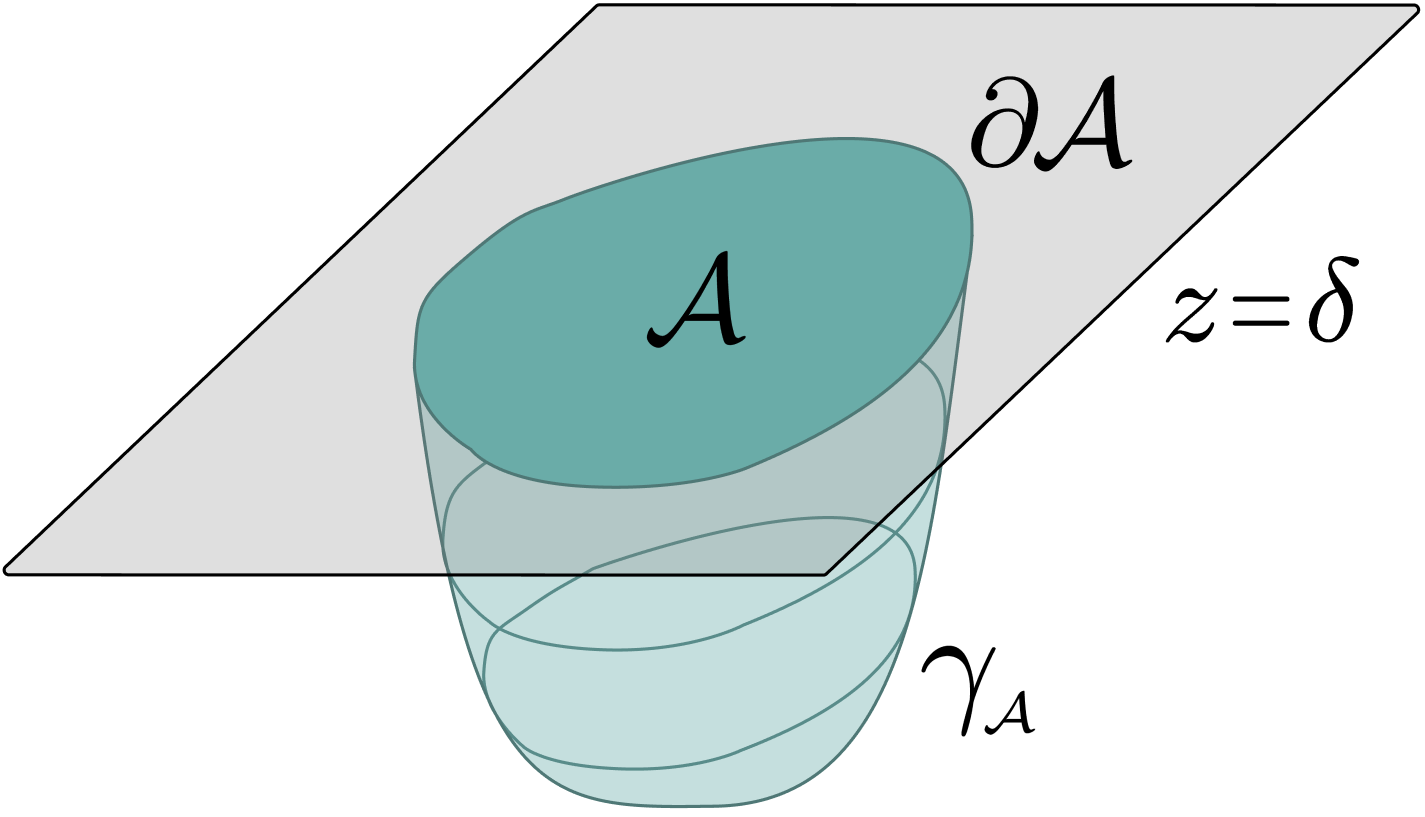
\includegraphics[width=0.25\textwidth]{../imatges/EE_AdS-CFT.png}
\caption{Region $A$ (dark blue) and its boundary $\partial A$ inside a $z=\delta$ AdS slide (grey) and its respective $\gamma_A$ (light blue) inside the AdS spacetime.}
\label{fig:EE_AdS-CFT}
\end{wrapfigure}

The Ryu-Takayanagi formula is valid for generic systems, and provides a hint on how the geometry of spacetime can emerge from mere quantum information. 

As one can verify, the Ryu-Takayanagi formula for a ($d+1$)-dimensional anti-de Sitter reproduces the expected general behaviour of the entanglement entropy (Eq.~\ref{eq:EE}) for a $d$-dimensional conformal field theory \cite{}. Let us see this explicitly with an example.


\subsection{Entanglement Entropy for a Disk in CFT$_3$} \label{ss:EE-disk}

In this section, we compute the entanglement entropy for a circular region in a holographic CFT$_3$ dual to Einstein gravity, to see if it is obtained the general expression of the EE for a QFT.

Let $A$ be a disk-shaped region of radius $R$ defined in the conformal boundary of an AdS$_4$. This 2-dimensional region is defined in polar coordinates as
\eq{1A}{
    A = \{ ( r, \theta, z, t ) \ | \ t = 0, z = \delta, r \le R \}
}
The corresponding surface of minimal area $\gamma_A$ of the region $A$, defined in the bulk and adjacent to $\partial A$, is parametrized as:
\eq{1gA}{
    \gamma_A = \{ ( r, \theta, z, t ) \ | \ t = 0, z = f (r, \theta) \} \ ,
}
where $f(r,\theta)$ is a certain function we need to identify. There is no property on the AdS spacetime theory that could prevent the symmetry of $\partial A$ on the coordinate $\theta$ from being transfered to $\gamma_A$. Hence, $z=f(r)$.

The metric corresponding to AdS$_4$ spacetime reads
\eq{1Ametric}{
    \mathrm{d}s^2_{\text{AdS}_4} = g_{\mu \nu} \mathrm{d}x^\mu \mathrm{d}x^\nu = 
    \frac{L^2}{z^2} [ -\mathrm{d}t^2 + \mathrm{d}z^2 + \mathrm{d}r^2 + r^2 \mathrm{d}\theta^2 ] \ .
}
The induced metric of the surface $\gamma_A$ reads:
\eq{1gammaAmetric}{
    \mathrm{d}s^2_{\gamma_A} = h_{i j} \mathrm{d}x^i \mathrm{d}x^j = 
    \frac{L^2}{f(r)^2} \left[ \left( 1+ \dot{f}(r)^2 \right) \mathrm{d}r^2 + r^2 \mathrm{d}\theta^2 \right] \ ,
}
being $\mathrm{d}z = \partial_\rho z \, \mathrm{d}x^\rho = \partial f(r)_r \, \mathrm{d}r = \dot{f}(r) \, \mathrm{d}r$. The determinant of the induced metric will be
\eq{1h}{
    h = \left( \frac{L}{f(r)} \right) ^4 r^2 ( 1 + \dot{f}(r)^2 ) \ .
}
The minimal value of the integral over the polar coordinates of the square root of the induced metric will correspond to the area of $\gamma_A$. So, by the Ryu-Takayanagi formula, the entanglement entropy related to the region $A$ will be
\eqgat{1EEA}{
    S_A = \frac{1}{4G} \, \text{min} \int_{\gamma_A} \sqrt{h} \ \mathrm{d}x^\rho \nonumber \\
    = \frac{\pi L^2}{2G} \, \text{min} \int_r \mathrm{d}r \frac{r}{f(r)^2} \sqrt{ 1 + \dot{f}(r)^2 } \ .
}
The interior of this final definite integral looks like some type of Lagrangian $\calL [r,f(r),\dot{f}(r)]$, whose Euler-Lagrange equation reads:
\eqgat{1EL}{
    \frac{\partial \calL}{\partial f} - \frac{\mathrm{d}}{\mathrm{d}r} \left[ \frac{\partial \calL}{\partial \dot{f}} \right] = 0 \nonumber \\
    \longrightarrow \left( 1+\dot{f}^2 \right) \left( -2r-f\dot{f}-rf\ddot{f} \right) + rf\dot{f}^2\ddot{f} = 0 \ .
}
One can prove that $f(r) = \sqrt{R^2 - r^2}$ is solution of the previous relation and corresponds to the function that minimizes the functional of the entanglement entropy and connects to the boundary region $A$. Hence, the surface of minimal area is found to be a half sphere.

To compute the integral of the EE expression, we should first determine its limits. The inferior bound corresponds to the lower part of the half sphere inside the bulk, where $r_\text{min}=0$. The superior bound corresponds to the connexion of the surface with the conformal boundary, that is, $z=\delta=\sqrt{R^2-r_\text{max}^2}$. Thus, the entanglement entropy of the disk will be
\eqgat{1sol}{
    S_A = \frac{\pi L^2}{2G} \, \text{min} \int_0^{\sqrt{R^2-\delta^2}} \mathrm{d}r \frac{r}{f(r)^2} \sqrt{ 1 + \dot{f}(r)^2 } = \nonumber \\
    = \frac{\pi L^2}{2G} \frac{R}{\delta} - \frac{\pi L^2}{2G} \ ,
}
that is equivalent to the general expression for the entanglement entropy in a 3-dimensional QFT, finally finding that
\eq{F}{
    s_\text{univ} = \frac{\pi}{2} \frac{L^2}{G} \ .
}
% ¿Poner algo sobre la importancia de esta constante?


\subsection{Strong subadditivity} \label{ss:SS}

The \textit{strong subadditivity} \cite{headrick_holographic_2007} is a fundamental general property of EE. Defines relations between entanglement entropies of two subsystems $A$ and $B$, and its union $A \cup B$, intersection $A \cap B$, and relative complements $A \setminus B$ and $B \setminus A$ (Fig.~\ref{fig:SS}):
\eqgat{EE_strong-subadd}{
    S(A) + S(B) \ge S(A \cup B) + S(A \cap B) \ , \nonumber \\
    S(A) + S(B) \ge S(A \setminus B) + S(B \setminus A) \ .
}

\begin{wrapfigure}[13]{r}{0.25\textwidth}
    \centering
    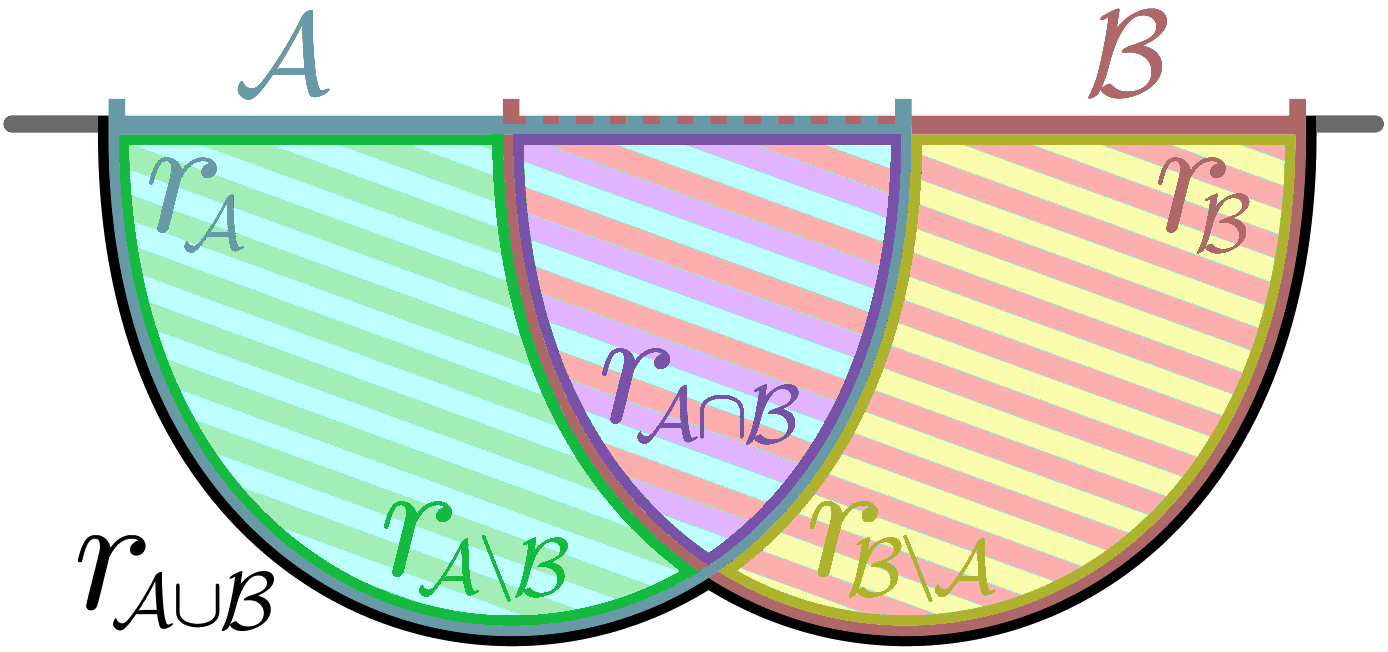
\includegraphics[width=0.25\textwidth]{../imatges/SS_D.png}
\caption{Representation of the bulks $r_A$ and $r_B$ corresponding to two subsystems $A$ and $B$, and their union, interception, and relative complements.}
\label{fig:SS}
\end{wrapfigure}

This properties are present in any quantum mechanical many-body theory. An important test of the validity of the Ryu-Takayanagi formula (Eq.~\ref{eq:EE_RT}) is whether it fulfills this property.

Let's start poving the first inequality. The regions of the bulks corresponding to the regions $A$ and $B$ will be defined as $r_A$ and $r_B$. Their union and interception will be $r_{A \cup B} = r_A \cup r_B$ and $r_{A \cap B} = r_A \cap r_B$. The surfaces boundaring this regions will be decomposed as
\eq{SS_dr-1}{
    \partial r_{A \cup B} = (A \cup B) \cup \gamma_{A \cup B} \ , \ \partial r_{A \cap B } = (A \cap B) \cup \gamma_{A \cap B} \ .
}
It is clear that $\gamma_{A \cup B}$ and $\gamma_{A \cap B}$ are connected to $\partial (A \cup B)$ and $\partial (A \cap B)$, respectively, but nothing says that they are their related surfaces of minimal area $\gamma^{\text{min}}_{A \cup B}$ and $\gamma^{\text{min}}_{A \cap B}$: they are upper bounds. This proves that
\eq{SS_gamma-1}{
    \gamma_A + \gamma_B = \gamma_{A \cup B} + \gamma_{A \cap B} \ge \gamma^{\text{min}}_{A \cup B} + \gamma^{\text{min}}_{A \cap B} \ ,
}
and, therefore, using the Ryu-Takayanagi formula (Eq.~\ref{eq:EE_RT}), the first inequality of Eq.~\ref{eq:EE_strong-subadd}.

Regarding the second inequality, let's define the bulk regions exclusive of $A$ and $B$: $r_{A \setminus B}$ and $r_{B \setminus A}$, respectively. The surfaces boundaring this regions will be decomposed as
\eq{SS_dr-2}{
    \partial r_{A \setminus B} = (A \setminus B) \cup \gamma_{A \setminus B} \ , \ \partial r_{B \setminus A } = (B \setminus A) \cup \gamma_{B \setminus A} \ .
}
Again, it is clear that $\gamma_{A \setminus B}$ and $\gamma_{B \setminus A}$ correspond to upper bounds for $\partial (A \setminus B)$ and $\partial (B \setminus A)$. Hence,
\eq{SS_gamma-2}{
    \gamma_A + \gamma_B = \gamma_{A \setminus B} + \gamma_{B \setminus A} \ge \gamma^{\text{min}}_{A \setminus B} + \gamma^{\text{min}}_{B \setminus A} \ ,
}
and the second inequality of \ref{eq:EE_strong-subadd} it is proven.

Using this simple geometric proof, it is shown that holography fulfills the strong subadditivity property that should be true in any quantum mechanical many-body system, playing the extra dimension in the holographic dual an essential role.


\subsection{Entanglement entropy for higher orders} \label{s:EE_HO}

It has been shown that the Ryu-takayanagi formula (\ref{eq:EE_RT}) as the entanglement entropy for holographic theories dual to Einstein gravity. Nevertheless, considering strings and not fields, and taking into account quantum properties, higher-order terms appear \cite{bueno_holographic_2021}.

For stringy corrections, the area functional needs to be modified, similarly to how the Bekenstein-Hawking formula for the entropy of a black hole (\ref{eq:BH}) is replaced by Wald formula \cite{iyer_properties_1994}. But replacing the functional of the entanglement entropy for the Wald's one does not work \cite{bueno_holographic_2021}. Additional ``anomaly'' terms corresponding to extrinsic curvatures of the generalized surface involving arbitrary contractions of Riemann tensors and metrics are required \cite{dong_holographic_2014}. In the anomaly term, each of the Riemann tensor components resulting has to be split into summatories of different weighted terms. The way that these terms are weighted is non-unique, leading to the so-called \textit{splitting problem}.

One can also consider corrections on the Ryu-Takayanagi formula related to quantum mechanical effects in the bulk \cite{faulkner_quantum_2013}. This quantum corrections are essentially given by the entanglement entropy between the bulk bounded by the minimal area surface and the outside region. One can see the bulk region as an effective field theory itself living on a fixed background geometry and compute its entanglement entropy as in any quantum field. One has to be cautious and do not confuse this entanglement entropy with the one computed by the Ryu-Takayanagi formula, which is intended to be generalized.


\section{Duality with Einstein field equations} \label{s:EQ}


\subsection{First law of entanglement entropy} \label{ss:FLEE}

The \textit{first law of entanglement entropy} is a generalization of the first law of thermodynamics for any arbitrary small perturbation, quantum state or subsystem.

For a small perturbation of a quantum field theory state $\ket{\psi(\varepsilon)}$ to the initial state $\ket{\psi(0)}$, the First Law of Entanglement Entropy is defined as
\eq{FLEE}{
    \delta S_A = \frac{\mathrm{d}}{\mathrm{d} \varepsilon} S_A = \frac{\mathrm{d}}{\mathrm{d} \varepsilon} \abs{H_A} = \frac{\mathrm{d}}{\mathrm{d} \varepsilon} \tr (H_A \rho_A) \equiv \delta E_{calA}
}
for the entanglement entropy of a subsystem $A$ \cite{fareghbal_first_2019}. The modular Hamiltonian $H_A$ is independent of the perturbation, and is defined by
\eq{modularH}{
    \rho_A (\varepsilon) = e^{-H_A}.
}

When $H_A$ is a local operator, $\rho_A$ can be mapped to a thermal one, $\rho_{\calH}$, by a unitary transformation, being the resultant entropy thermal. Hence, $\rho_{\calH}$ can be written as
\eq{modularH2}{
    \rho_{\calH} = \frac{e^{-H_{\calH}}}{\tr (e^{-H_{\calH}})} \ ,
}
where $H_{\calH}$ is the associated charge of the so-called modular flow $\xi$.

In the holographic description, it has been shown that writing both sites of the first law of entanglement entropy in terms of the corresponding bulk parameters leads to a constraint on the bulk geometry that is exactly the Einstein field equations \cite{fareghbal_first_2019}. If this was an intrinsic property of any gauge/gravity theory, one could use entanglement entropy in an arbitrary field theory to find a dual gravitational geometry.


\subsection{First law of entanglement entropy applied to holography} \label{ss:FLEE_H}

---


\section{Conclusions} \label{s:Conclusions}

---


\begin{acknowledgments}

---

---

---
    
\end{acknowledgments}



\bibliography{TFG.bib}



\end{document}